% -*- coding: utf-8 -*-
\documentclass[t]{beamer} % Add option ``handout'' to produce handouts
\usepackage[english, ngerman]{babel}
\usepackage[utf8]{inputenc}
\usepackage[T1]{fontenc}
\usepackage{pxfonts}

\usetheme[german, informal]{UZH} % Available options: german (default), english,
                                 % informal (default), formal

\mode<presentation>
{
  \setbeamercovered{transparent}

  % For gray section slides
  \AtBeginSection[]{%
    \setbeamercolor{background canvas}{bg=UZHgray}
    \setbeamercolor{frametitle}{bg=UZHgray, fg=white}
    \begin{frame}<beamer>[plain]
      \frametitle{\insertsection}
    \end{frame}
    \setbeamercolor{background canvas}{bg=white}
    \setbeamercolor{frametitle}{bg=white, fg=UZHblue}
  }
}

\mode<handout>
{
  \usepackage{pgfpages}
  \pgfpagesuselayout{2 on 1}[a4paper, border shrink=5mm]
}

\newcommand{\first}[1]{\emph{#1}}
\newcommand{\q}[1]{\iflanguage{ngerman}{\flqq#1\frqq}{``#1''}}

%%%%%%%%%%%%%%%%%%%%%%%%%%%%%%%%%%%%%%%%%%%%%%%%%%%%%%%%%%%%%%%%%%%%%%%%%%%%%%%

\title[Sprachvarianten]{Sprachvarianten des Deutschen im Zeitraum 1600 bis heute}
\subtitle{Vorlesung: Sprachtechnologie für historische Dokumente: Konzepte und Anwendungen (HS~2011)}
\institute[Institut für Computerlinguistik]{Institut für Computerlinguistik\\
Dozenten: Dr. Cerstin Mahlow, Dr.-Ing. Michael Piotrowski}
\author[Hafner, Marques~Madeira, Baumgartner]{Simon Hafner, Hernani Marques~Madeira, Reto Baumgartner}
\date{\today}



\begin{document}
% NOTE: Do not enclose \maketitle in a frame, or switching to the
%       normal templates will not work!
\maketitle

\section*{Problemstellung}

\begin{frame}
\thispagestyle{empty}
  \frametitle{Problemstellung}
  Erkennung der Entstehungszeit \\
  historischer Texte nach 1600

  \begin{itemize}
  \item Im Rahmen des Projekts OLdPhras\footnote{URL: \url{http://colloc.germa.unibas.ch/oldphras/ (17.12.2011)}}
  \item Unser Code (public domain) verfügbar. URL: \url{https://github.com/2mh/OLdPhras-langvar}
  \item Lösungsansatz: Mit Hilfe eines n"=Gramm"=Sprachmodells (statistisch)
  \item Frage: Wo liegen die besten Resultate -- bei welcher n"=Gramm"=Ordnung, zeichen"= oder wortbasiert?
  \end{itemize}
\end{frame}

\section{Trainingskorpus (Reto Baumgartner)}

\begin{frame}
\thispagestyle{empty}
  \frametitle{Daten für das Trainingskorpus}
  \begin{itemize}
  \item Deutsches Textarchiv\footnote{URL: \url{http://www.deutschestextarchiv.de/} (17.12.2011)}\\
  \vspace*{1ex}
  
  \item Bereich Literatur
  \vspace*{1ex}
  
  \item Nach den Regeln der Text Encoding Initiative (TEI-P5\footnote{URL: \url{http://www.tei-c.org/index.xml} (17.12.2011)})
  \end{itemize}
\end{frame}

\begin{frame}
  \frametitle{TEI-Format}
  Mehrere Werke in einem XML"=File
  \vspace*{1ex}
  
  Einzelne Werke repräsentiert durch Knoten mit dem Tag «TEI»
  \begin{itemize}
  \item Literaturgenre:
    \begin{itemize}
    \item \texttt{TEI/teiHeader/profileDesc/textClass/keywords/term}    
    \item \texttt{prose}, \texttt{drama}, \texttt{verse}
    \end{itemize}
    \vspace*{1ex}
    \pause
    
  \item Erstellungsdatum: 
    \begin{itemize}
    \item \texttt{TEI/teiHeader/profileDesc/creation/date}   
    \item \texttt{notBefore=''1840'' notAfter=''1902''} (z. B. bei Texten von Emile Zola, geb. 1840, $\dagger$ 1902)
    \end{itemize}
    \vspace*{1ex}
    \pause
    
  \item Text:\\
    \begin{itemize}
    \item \texttt{TEI/text}
    \end{itemize}
  \end{itemize}
\end{frame}

\begin{frame}
  \frametitle{Werkzeug zur Erstellung des Trainingskorpus}
  \texttt{korpusbastler.py}
  \vspace*{1ex}
  
  In Python codiert
%  \vspace*{1ex}
%  
%  Einsetzbar ab Python 3.2
%  
%  Gründe dazu:
%  \begin{itemize}
%  \item Eher neue Funktion \texttt{xml.etree.cElementTree.itertext()}
%  \item Einfachere Arbeit mit Encodings ab Python 3.x
%  \end{itemize}
\end{frame}

\begin{frame}
  \frametitle{Werkzeug zur Erstellung des Trainingskorpus}
  Für jedes enthaltene Werk:
  
  \begin{itemize}
  \item Literaturgenre:
    \begin{itemize}
    \item Weiterverarbeitung der Genres \texttt{prose}, \texttt{drama} 
    \item Keine Textextraktion bei Genres wie \texttt{verse}
    \end{itemize}
    \vspace*{1ex}
    \pause

  \item Erstellungsdatum:
    \begin{itemize}
    \item \texttt{notBefore, notAfter}: Lebensdaten des Autors
    \item Mögliches Erstellungsjahr: Mitte zwischen den Jahren 
    \item Einteilung in Korpora nach halben Jahrhunderten mithilfe des Erstellungsjahres
    \end{itemize}
    \vspace*{1ex}
    \pause
    
  \item Text:
    \begin{itemize}
    \item Extraktion des Textes auf allen Tiefen
    \item Mit \texttt{xml.etree.cElementTree.itertext()}
    \item Schreiben in entsprechende Korpusdateien
    \end{itemize}
  \end{itemize}
\end{frame}

\begin{frame}
  \frametitle{Trainingskorpora für die Sprachmodelle}
  \begin{tabular}{lrl}
  Sprachstufe & \multicolumn{2}{l}{Anzahl Wörter im Korpus}
  \vspace*{1ex}\\
  1600--1650 & 2'574'487 &(rund 16 MB)\\
  1650--1700 & 5'652'759 &(rund 34 MB)\\
  1700--1750 & 2'809'613 &(rund 18 MB)\\
  1750--1800 & 9'101'048 &(rund 56 MB)\\
  1800--1850 & 19'325'579 &(rund 118 MB)\\
  1850--1900 & 27'389'361 &(rund 169 MB)\\
  1900--     & 2'396'123 &(rund 15 MB)
  \end{tabular}
\end{frame}

\section{Testkorpus}

\begin{frame}
  \frametitle{Testkorpora}
  \begin{itemize}
  \item Aus \url{http://de.wikisource.org/}\pause
  \vspace*{1ex}
  \item 100 Sätze pro Sprachstufe\pause
  \item d.\,h. 20 Sätze pro Jahrzehnt\pause
  \item Ausnahme bei Testsatz ab 1900 (rund 10 Sätze je Jahrzehnt)\pause
  \vspace*{1ex}
  \item Genres entsprechen dem Trainingskorpus
  \end{itemize}  
\end{frame}

\section{Sprachmodelle (Hernani Marques)}

% n-Gramm
\begin{frame}
  \frametitle{n-Gramm-Wahrscheinlichkeiten (bedingt)}
  \begin{itemize}
  \item Basierend auf Übungen in PCL3-HS11\pause
  \vspace*{1ex}
  \item Zeichenbasierte n-Gramm-Modelle: 1- bis 6-Gramme\pause
  \item Somit: Insg. 6 n-gramm-Modelle (7 Sprachvarianten abbildend)\pause
  \item Smoothing für unvorhandene Sequenzen (arbiträr): $10^(-8)$
  \vspace*{1ex}
  \end{itemize}  
\end{frame}

% 
\begin{frame}
  \frametitle{Werkzeug zum Training der Daten}
  \texttt{langMod.py}
  \begin{itemize}
  \item Funktion \emph{generate\_ngrams()} liefert n-Gramme zurück (zeichen- oder wortbasiert); ist ein Generator\pause
  \item Klasse \emph{LM} speichert (bedingte) n-Gramm-Wahrscheinlichkeiten pro Sprachvariante\pause
  \item Klasse \emph{MLM} speichert LM-Modelle
  \vspace*{1ex}
  \end{itemize}  
\end{frame}

\begin{frame}
  \frametitle{Training der Daten}
  \begin{itemize}
  \item \texttt{timeRanges = [ "1600\_1650", "1650\_1700", "1700\_1750", "1750\_1800", "1800\_1850", "1850\_1900", "1900\_2010"]}
  	\begin{itemize}
  	\item Training von sieben (deutschen) Sprachvarianten in 50er Jahre Blöcke; Ausnahme bei modernen Sprache
  	\end{itemize}\pause
  \item \texttt{gramTypes = [''Z'',''W''] \# symbol-based (Z) and word-based (W)}
  	\begin{itemize}
   	\item n-Gramm-Arten: Zeichenbasiert, wortbasiert
  	\end{itemize}\pause
  \item \texttt{gramOrders = range(1,7) \# for n-gram order 1-6}
  	\begin{itemize}
   	\item n-Gramm-Ordnungen: 1-6 (5 und 6 haben eine (sehr) kritische Komplexität)
  	\end{itemize}
  \end{itemize}  
\end{frame}


% 
\begin{frame}
  \frametitle{Werkzeug zur Sprachidentifikation}
  \texttt{langMod.py}
  \begin{itemize}
  \item Funktion \emph{accuracy()} liefert wahrscheinlichste Sprachvariante für eine Testzeile zurück
   \begin{itemize}
    \item Ein Objekt der Klasse \texttt{MLM} führt wahrscheinlichste Sprache für diese Zeile an
   \end{itemize}\pause
  \item Anhand 100 Testzeilen (Dateien \emph{e100-*}) von Sätzen der jeweiligen Sprachvariante messen wir die Genauigkeit (Anzahl Treffer / 100)
  \end{itemize}  
\end{frame}

\section{Ergebnisse (Simon Hafner)}
\begin{frame}
 \frametitle{Ergebnisse}
 \tiny
  \begin{tabular}{l|ccccccc}
    & 1600-1650 & 1650-1700 & 1700-1750 & 1750-1800 & 1850-1900 &
    1900-2010 \\
    \hline
    Unigramm & 0.54 & 0.5 & 0.42 & 0.09 & 0.03 & 0.07 & 0.16 \\
    Bigramm & 0.73 & 0.54 & 0.31 & 0.25 & 0.38 & 0.61 & 0.09 \\
    Trigramm & 0.65 & 0.68 & 0.22 & 0.46 & 0.46 & 0.52 & 0.16 \\
    4-gramm & 0.66 & 0.8 & 0.2 & 0.5 & 0.44 & 0.49 & 0.12 \\
    5-gramm & 0.53 & 0.82 & 0.12 & 0.46 & 0.45 & 0.6 & 0.01 \\
    6-gramm & 0.39 & 0.86 & 0.1 & 0.32 & 0.53 & 0.63 & 0.0 \\
  \end{tabular}
\end{frame}

\begin{frame}
  \begin{figure}[ht]
    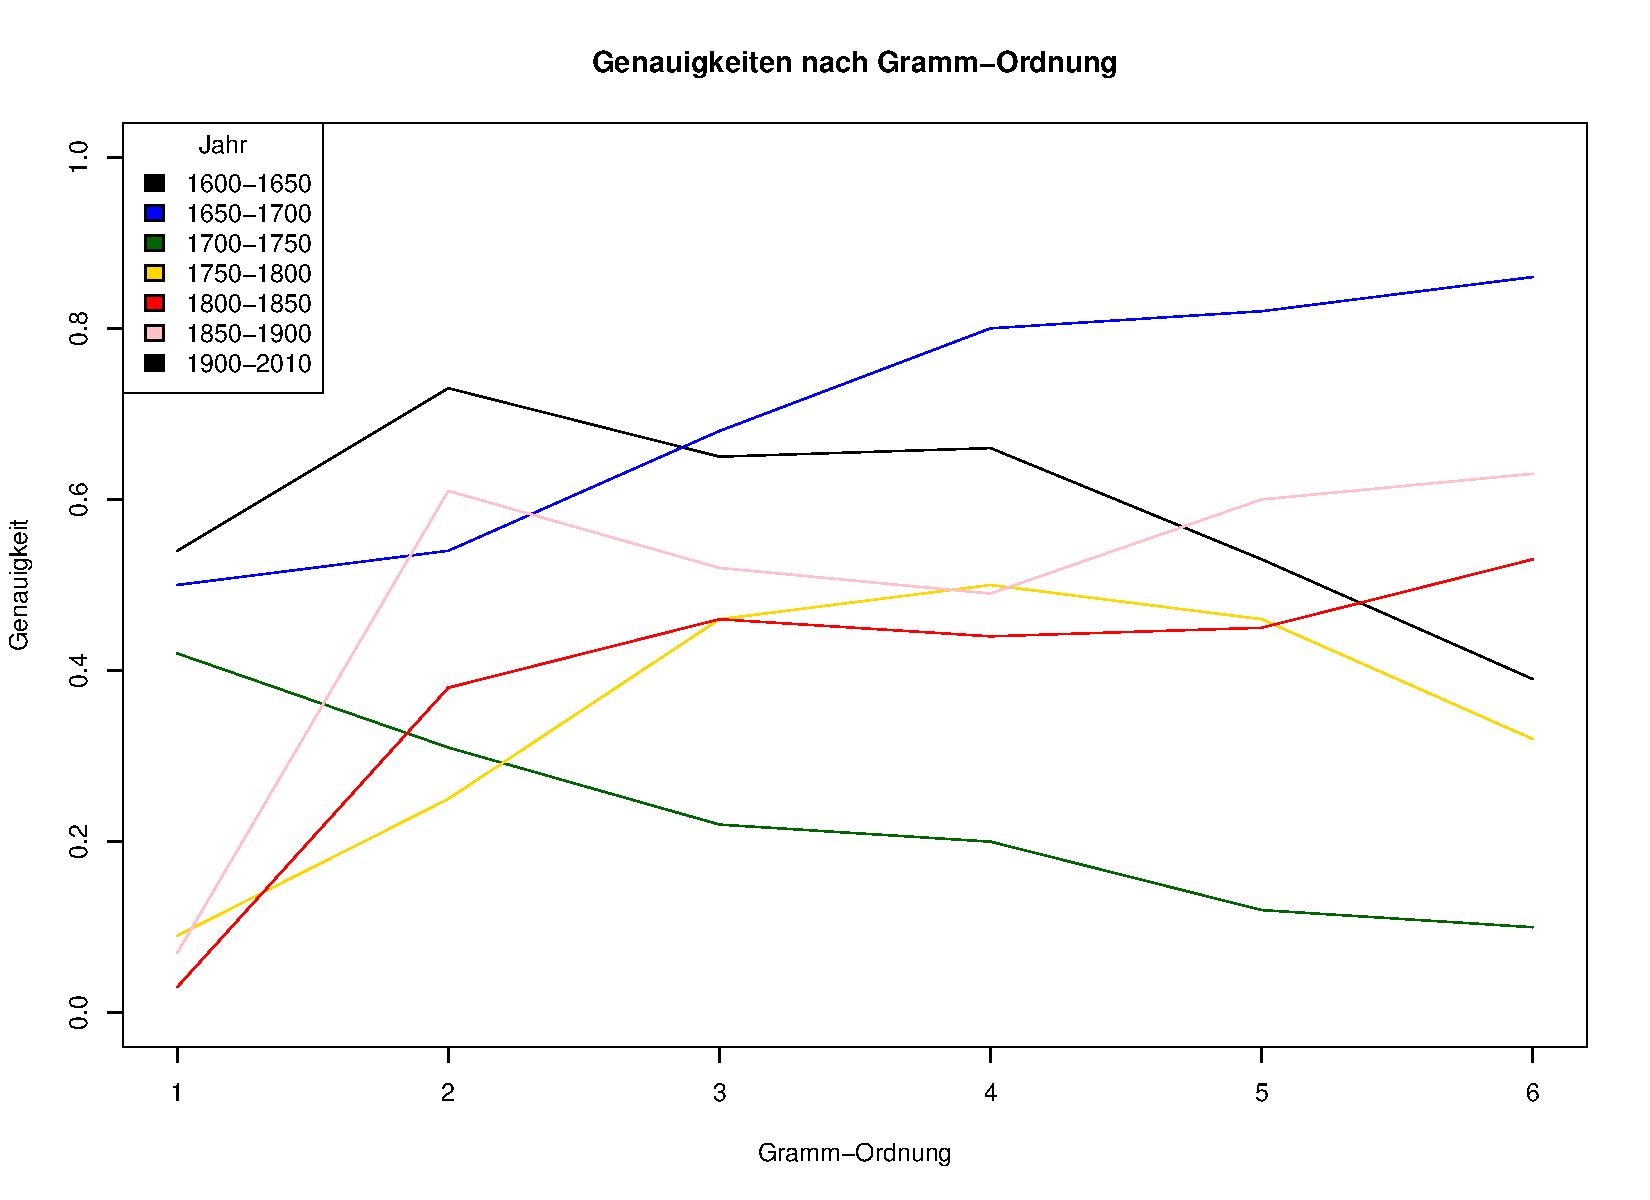
\includegraphics[width=1\textwidth]{Jahr}
  \end{figure}
\end{frame}

\begin{frame}
  \begin{figure}[ht]
    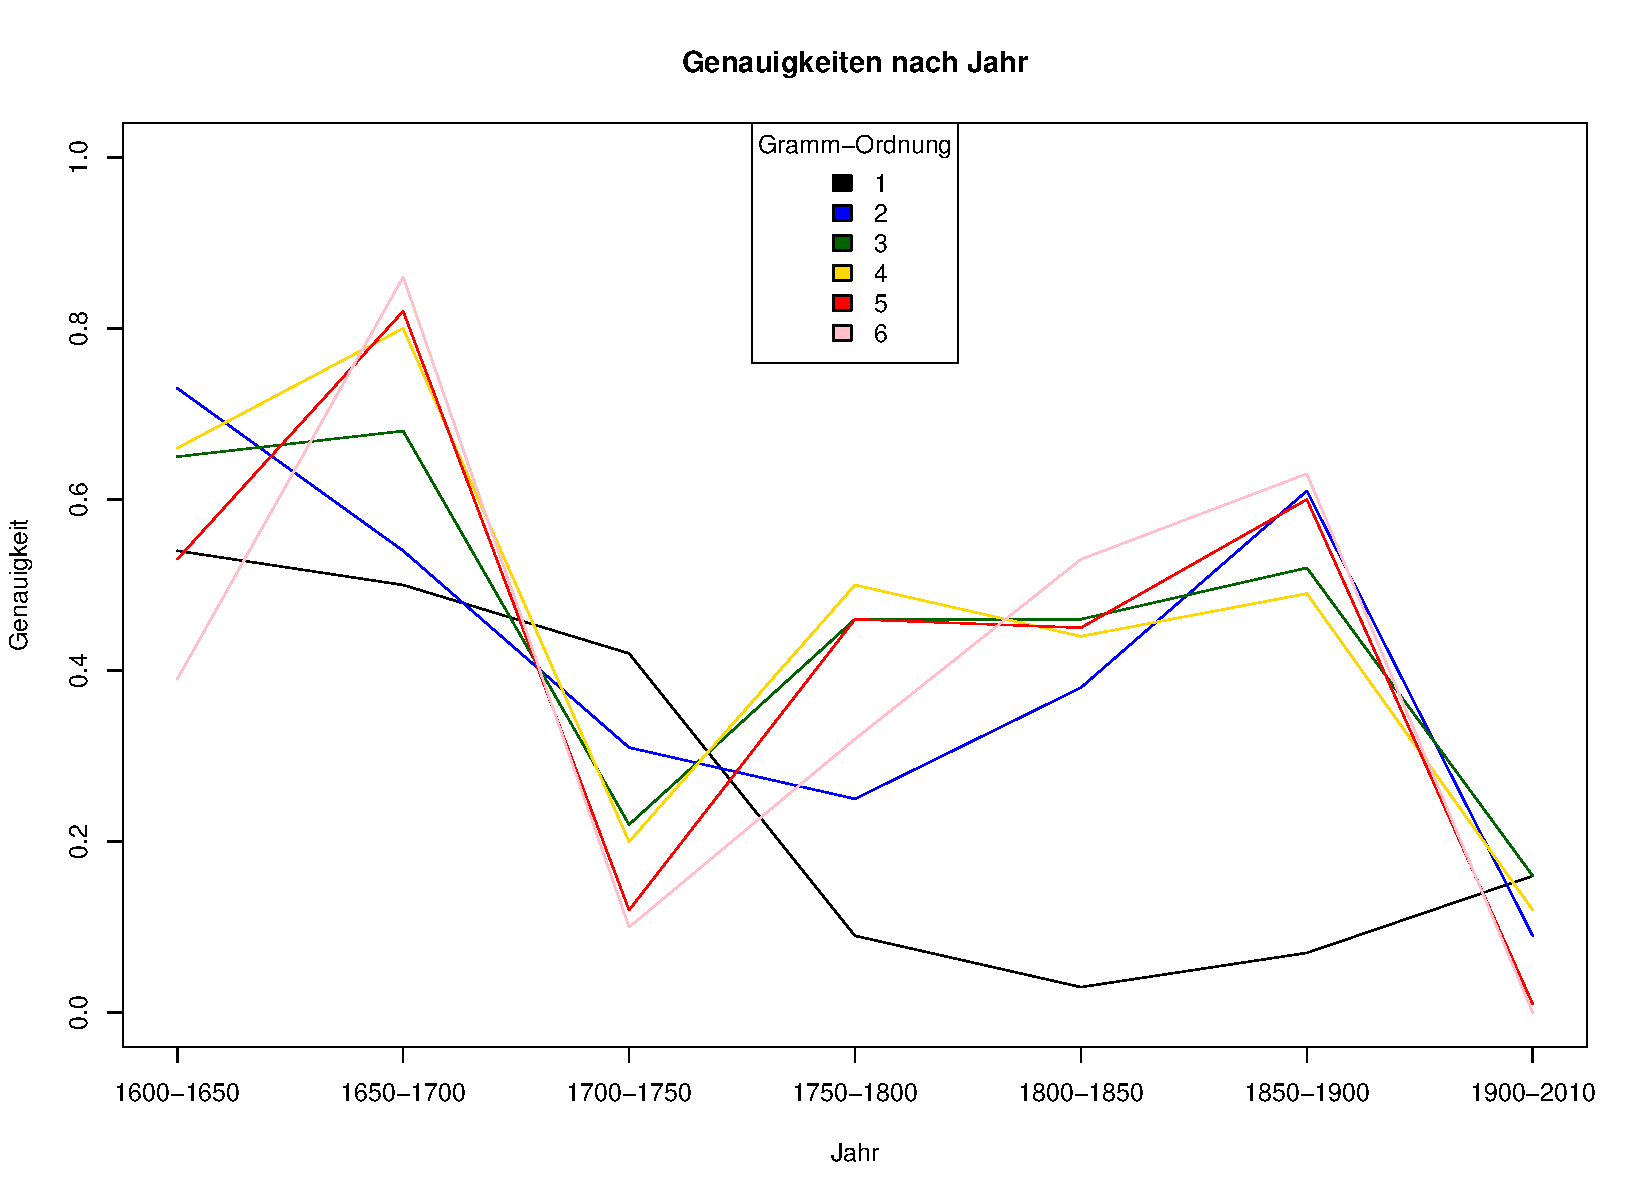
\includegraphics[width=1\textwidth]{Gramm}
  \end{figure}
\end{frame}

\section{Verbesserungsmöglichkeiten (Simon Hafner)}
\begin{frame}
  \frametitle{Trainingskorpus}
  \begin{itemize}
  \item Menge Sprachmaterial (ungleich verteilt aktuell)\pause
  \item Textsorten (potenziell ungleich verteilt)\pause
  \item Nachbearbeitung des Sprachmaterials u. U. nötig\pause
  \end{itemize}  
\end{frame}

\begin{frame}
  \frametitle{Testsätze}
  \begin{itemize}
  \item Auswahl ist (zufällig) auf Wikisource erfolgt\pause
  \vspace*{1ex}
  \item Sätze vs. Absätze (letztere (= länger) liefern akuratere Resultate)\pause
  \item Textsorten (potenziell ungleich verteilt, insb. ab 1900 bis heute)\pause
  \begin{itemize}
   \item Rechtliche Texte dominieren ab 1940er auf Wikisource
   \item Andere Textsorten tendenziell nicht public domain
  \end{itemize}
  \end{itemize}  
\end{frame}

\begin{frame}
<<<<<<< HEAD
  \frametitle{Ergebnisse}
  \tiny\begin{tabular}{l|ccccccc}
    & 1600-1650 & 1650-1700 & 1700-1750 & 1750-1800 & 1800-1850 & 1850-1900 &
    1900-2010 \\
    \hline
    Unigramm & 0.54 & 0.5 & 0.42 & 0.09 & 0.03 & 0.07 & 0.16 \\
    Bigramm & 0.73 & 0.54 & 0.31 & 0.25 & 0.38 & 0.61 & 0.09 \\
    Trigramm & 0.65 & 0.68 & 0.22 & & 0.46 & 0.46 & 0.52 & 0.16 \\
    4-gramm & 0.66 & 0.8 & 0.2 & 0.5 & 0.44 & 0.49 & 0.12 \\
    5-gramm & 0.53 & 0.82 & 0.12 & 0.46 & 0.45 & 0.6 & 0.01 \\
    6-gramm & 0.39 & 0.86 & 0.1 & 0.32 & 0.53 & 0.63 & 0.0 \\
  \end{tabular}
\end{frame}

\section{Projektideen (Simon Hafner)}

\begin{frame}
  \frametitle{Kritikpunkte}
  \begin{itemize}
  \item Weitere statistische Masse einführen\pause
  \item Smoothing-Algorithmus\pause
  \end{itemize}  
\end{frame}

\begin{frame}
  \frametitle{Codekomplexität/-Ausführungsgeschwindigkeit}
  \begin{itemize}
  \item Das Trainieren von Daten dauert lange (insb. bei Wort-n-Grammen)\pause
  \vspace*{1ex}
  \item Multiprozessor-Support einbauen\pause
  \item Algorithmische Verbesserungen (Zeit-/Raumkomplexität)\pause
  \item Andere Programmiersprache verwenden\pause
  \vspace*{1ex}
  \end{itemize}  
\end{frame}

\section{Fragen}

\end{document}

%%% Local variables:
%%% TeX-PDF-mode: t
%%% End:
